In 1982, a new neutral-beam injection heating system was install in the ASDEX tokamak, which pushed the device into a new realm.
A new level of energy confinement time was achieved, measured to be a factor of 2 or more than what was expected.
This state of operation was coined the high-confinement (H-) mode, and is now considered necessary for the future of nuclear fusion as an energy source \cite{arnoux_how_2009} \cite{wagner_development_1984}.
With this new level of energy confinement, the community got one step closer to economic fusion power plants.
The details of this transition, however, are not fully understood.

\section{Characteristics of L- and H-Mode}
Transport of particles and energy in tokamaks has been discovered to be significantly dominated by anomalous (turbulent) transport, which is generally assumed to be generated by turbulence, driven by micro-instabilities.
Low-confinement mode, L-mode, is dominated by this transport at the edge.
The formation of H-mode is due to the suppression of this turbulent transport at the edge of the plasma; thus is categorized as a transport barrier.
The plasma edge is defined to be the thin boundary layer of the plasma just inside the separatrix.


\begin{figure}[b] % L-H-modes compare
\begin{minipage}{0.49\linewidth}
	\centering
	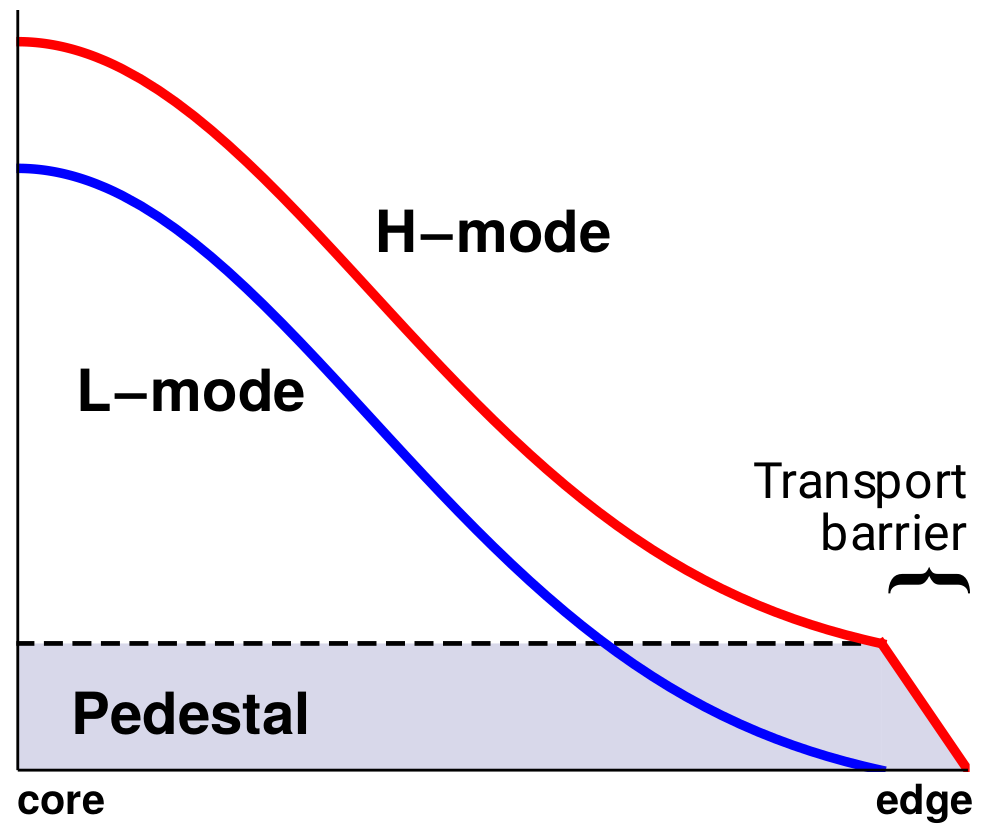
\includegraphics[width=0.8\textwidth]{../Graphics/L-mode_H-mode_compare.png}
\end{minipage}
\hfill
\begin{minipage}{0.49\linewidth}
	\caption{A comparison of the radial pressure profiles of L-mode and H-mode.
	The profile of H-mode can be thought of as on a `pedestal,' in which the pressure profile is increase in the core.
	This is due to the transport barrier that is formed at the edge \cite{weymiens_bifurcation_2014}.}
	\label{fig:L-mode_H-mode_compare}
\end{minipage}
\end{figure}

H-mode is characterized by its pressure profile significantly raised compared to that of L-mode, and is said to sit on a `pedestal.'
Accordingly, there is a steep gradient in the pressure at the edge of the plasma, shown and compared to L-mode in Figure~\ref{fig:L-mode_H-mode_compare} \cite{weymiens_bifurcation_2014}.
This results in an increase temperature in the core.

\section{The L-H Transition}
The key feature that determines a divertor tokamak's operational mode is the amount of external heating power.
It is also important to note that limiter tokamaks are relegated to stay in L-mode, as H-mode is exclusive to tokamaks with divertors.
The transition can occur in one of three manners: sharp, smooth, and oscillatory.

\subsection{Bifurcation Theory and Hysteresis}
A bifurcation is defined to be a topological or qualitative change in a system when a small and smooth change of a parameter is made.
The dynamic behavior of the L-H transition correspond very closely to a few certain bifurcations.
Physically, the transition is a bifurcation in the turbulent transport at the edge of the tokamak.
Sharp and smooth transitions are features of the cusp bifurcation, a two-fold bifurcation \cite{weymiens_bifurcation_2014}. 
The topological norm form of this behavior is
\begin{equation}
	\dot{x} \,=\, a - bx - x^3
	\label{eq:sharp_bif}
\end{equation}

These two dynamics are distinguished only by density as the parameter .
The most common transition is the sharp transition, as the plasma parameters for it are more ideal for achieving fusion.
\TwoFig{../Graphics/Bif_3D.png}
	{Two codimension 1 fold bifurcations, with the parameter $b$ dictating the size of the hysteresis, until the bifurcations merge into a cusp \cite{weymiens_bifurcation_2014}.}
	{fig:Bif_3D}
	{../Graphics/3_transitions_single_simple.png}
	{Codimension 3 parameter space with the black line indicating the fold bifurcation. The parameter $b$ dictates the type of transition, including the size of the hysteresis in the sharp transition \cite{weymiens_bifurcation_2014}.}
	{fig:Bif_types}

The third type of transition dynamics is oscillatory, also known as dithering.
These oscillatory solutions will only occur in the region near the cusp bifurcation point.

Hysteresis is also commonly present in the system, in which the current state of the system depends on its history.
The threshold power for the H-L transition is significantly lower than that of the L-H transition, leading to a region in which there is a non-unique solution to the plasma state.


\section{Mechanisms}
The prevailing hypothesis for the overarching mechanism for H-mode is that high auxiliary power develops strong sheared plasma flow and suppresses transport \cite{freidberg_plasma_2007}.

The shear stress dissociates smaller turbulent structures, with their energy and momenta transferred to larger flows \cite{staps_backstepping_2017}.
%The $\mathbf{E}\times\mathbf{B}$-velocity shear, which has been modeled many times.

